\documentclass[11pt]{article}
\usepackage{enumerate}
\usepackage{fullpage}
\usepackage{fancyhdr}
\usepackage{amsmath, amsfonts, amsthm, amssymb}
\usepackage{graphicx}
\usepackage{wasysym}
\usepackage{bbm}

\setlength{\parindent}{0pt}
\setlength{\parskip}{5pt plus 1pt}
\pagestyle{empty}

%%%%%%%%%%%%%%%%%%%%%%%HEADER%%%%%%%%%%%%%%%%%%%%%%%%%%%%%%
\newcommand{\myname}{Shashank Singh\footnote{sss1@andrew.cmu.edu}
        \footnote{Machine Learning Department \& Department of Statistics}}
\newcommand{\myclass}{10-715 Advanced Introduction to Machine Learning}
\newcommand{\myhwnum}{3}
\newcommand{\duedate}{Wednesday, November 12, 2014}
%%%%%%%%%%%%%%%%%%%%%%%%%%%%%%%%%%%%%%%%%%%%%%%%%%%%%%%%%%%

%%%%%%%%%%%%%%%%%%%%CONTENT MACROS%%%%%%%%%%%%%%%%%%%%%%%%%
\renewcommand{\qed}{\quad \ensuremath{\blacksquare}}
\newcommand{\inv}{^{-1}}
\newcommand{\bv}{\mathbf{v}}
\newcommand{\bx}{\mathbf{x}}
\newcommand{\by}{\mathbf{y}}
\newcommand{\bff}{\mathbf{f}}
\newcommand{\bzero}{\mathbf{0}}
\newcommand{\bxi}{\boldsymbol{\xi}}
\newcommand{\boldeta}{\boldsymbol{\eta}}
\newcommand{\dist}{\operatorname{dist}}
\newcommand{\area}{\operatorname{area}}
\newcommand{\vspan}{\operatorname{span}}
\newcommand{\Gr}{\operatorname{Gr}} % graph of a function
\renewcommand{\sp}{\operatorname{span}} % span of a set
\newcommand{\sminus}{\backslash}
\newcommand{\E}{\mathbb{E}} % expected value
\newcommand{\F}{\mathcal{F}}
\renewcommand{\H}{\mathcal{H}}
\newcommand{\pr}{\mathbb{P}} % probability
\newcommand{\Var}{\operatorname{Var}} % variance
\newcommand{\Cov}{\operatorname{Cov}} % covariance
\newcommand{\tr}{\operatorname{tr}} % trace
\newcommand{\N}{\mathbb{N}} % natural numbers
\newcommand{\Z}{\mathbb{Z}} % integers
\newcommand{\Q}{\mathbb{Q}} % rational numbers
\newcommand{\R}{\mathbb{R}} % real numbers
\newcommand{\A}{\mathcal{A}}
\newcommand{\B}{\mathcal{B}}
\newcommand{\C}{\mathcal{C}} % compact functions
\newcommand{\K}{\mathbb{K}} % underlying field of a linear space
\newcommand{\Ran}{\mathcal{R}} % range of a linear operator
\newcommand{\Nul}{\mathcal{N}} % null-space of a linear operator
\renewcommand{\L}{\mathcal{L}} % bounded linear functions
\newcommand{\pow}[1]{\mathcal{P}\left(#1\right)} % power set of #1
\newcommand{\e}{\varepsilon} % \varepsilon
\newcommand{\wto}{\rightharpoonup} % weak convergence
\newcommand{\wsto}{\stackrel{*}{\rightharpoonup}} % weak-* convergence
\newcommand{\X}{\mathcal{X}}
\newcommand{\Y}{\mathcal{Y}}
\renewcommand{\P}{\mathbb{P}}   % probability
\newcommand{\ind}{\perp\!\!\!\perp} % independent
\newcommand{\bfK}{\mathbf{K}} % bold K
\newcommand{\bfJ}{\mathbf{J}} % bold J
\newcommand{\bfB}{\mathbf{B}} % bold B
%%%%%%%%%%%%%%%%%%%%%%%%%%%%%%%%%%%%%%%%%%%%%%%%%%%%%%%%%%%

\begin{document}
\thispagestyle{plain}

{\Large Homework \myhwnum, Problem 1} \\
Name: \myname \\
\myclass \\
Due: \duedate

\section{Gaussian Processes (Samy)}
\subsection{GP Implementation}
Results and code for GP regression, hyperparameter selection, and posterior
sampling are included below.
\subsubsection*{Results}
The plot for the $1D$ data set is shown in Figure \ref{fig:GP1}.
\begin{figure}[h!]
\centering
\quad\;
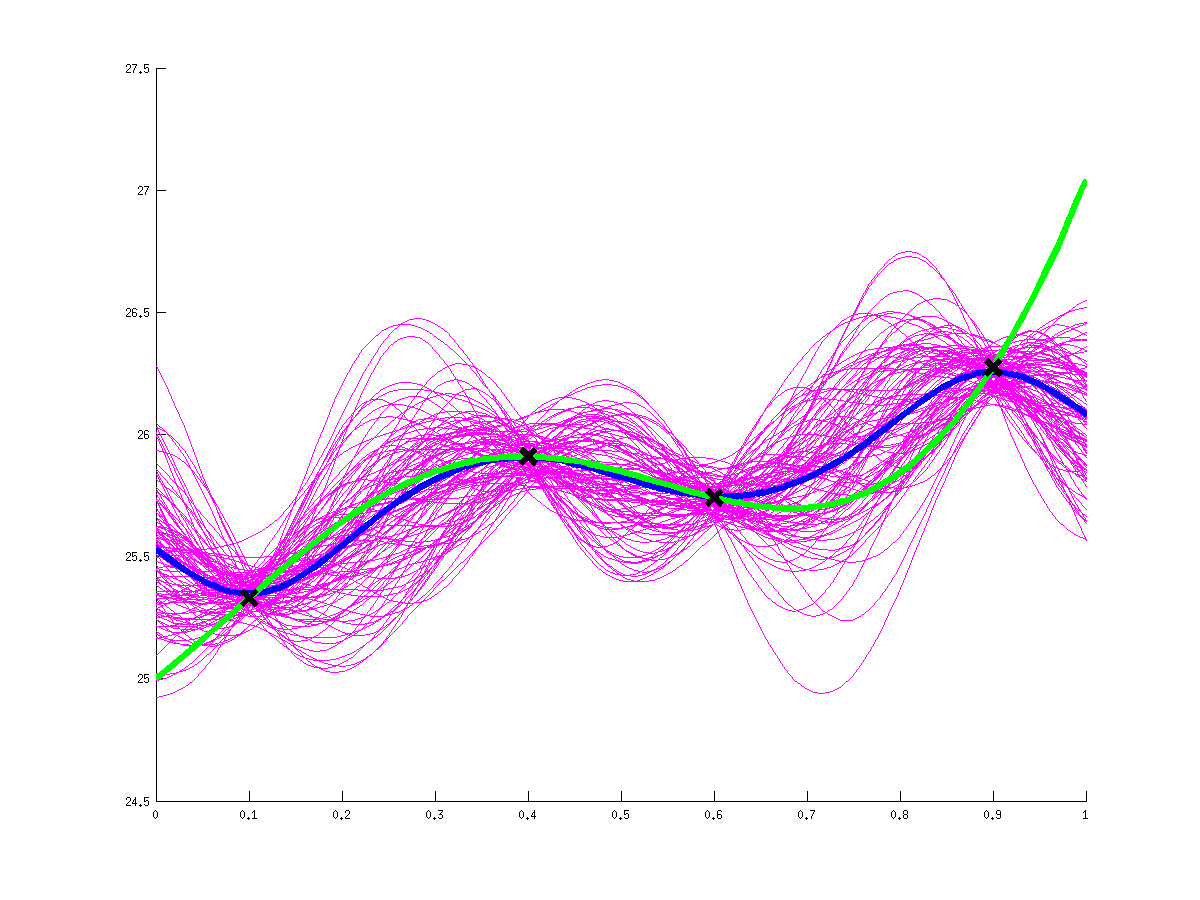
\includegraphics[width=0.75\linewidth]{GP1}
\vspace{-12mm}
\caption{True curve (green), posterior mean (blue), and $100$ samples (pink).}
\label{fig:GP1}
\end{figure}

The output on the CCPP data set was:
\begin{verbatim}
Error: 17.0268

ans =

  454.5271
  454.5271
  454.5271
  454.5271
  454.5271


ans =

    0.1000         0         0         0         0
         0    0.1000         0         0         0
         0         0    0.1000         0         0
         0         0         0    0.1000         0
         0         0         0         0    0.1000
\end{verbatim}
\subsection{Gradients using GPs}
\begin{enumerate}
\item \fbox{$[y,g_*]^T \sim \mathcal{N}(0, \Sigma)$,} where $\Sigma$ is the
block matrix
\[\mbox{\fbox{$\Sigma =
    \begin{bmatrix}
        \bfK    & \bfJ \\
        \bfJ^T  & \bfB
    \end{bmatrix}$.}}
\]
\item Using the formula for the conditional distribution of jointly Gaussian
variables given in the previous assignment, 
\[\mbox{\fbox{$g_* | y \sim \mathcal{N}(\bfJ^T \bfK\inv y, \bfB - \bfJ^T
\bfK\inv \bfJ)$.}}\]
\item The posterior mean $\E[y_* | y] = k_*^T \bfK\inv y$, where $k_* \in \R^n$
is the column vector whose $i^{th}$ entry is $k(x_*,x_i)$. Hence, since
$\bfK\inv$ and $y$ do not depend on $x_*$,
\[\nabla_{x_*} \E[y_* | y]
    = \left( \nabla_{x_*} k_*^T \right) \bfK\inv y
    = \bfJ^T K\inv y,
\]
by definition of $\bfJ$. This matches the mean from part 2. \qed
\item Suppose we want to estimate $Y(x_*)$ for some $x_* \in [a,b]$. Let
$\bfK,\bfJ$, and $\bfB$ be defined as above, but for $Y$ rather than $y$; that
is
\[\bfK = K(x_*,x_*), \quad
    \bfJ_i = \frac{\partial K(x_i,x_*)}{\partial x_i}
    \quad \mbox{ and } \quad
    \bfB_{i,j} = \frac{\partial^2 K(x_i,x_j)}{\partial x_i \partial x_j}
\]
(since $Y : \R \to \R$ but we are evaluating $y$ at $n$ points,
$\bfK \in \R^{1 \times 1}$, $\bfJ \in \R^{n \times 1}$ and
$\bfB \in \R^{n \times n}$). Then, $[y,Y(x_*)]^T \sim \mathcal{N}(0, \Sigma)$,
where $\Sigma$ is the block matrix
\[\Sigma =
    \begin{bmatrix}
        \bfB    & \bfJ \\
        \bfJ^T  & \bfK
    \end{bmatrix}.
\]
Hence, by the formula from the previous assignment, the posterior for $Y(x_*)$
is given by
\fbox{$Y(x_*) | y
    \sim \mathcal{N}(\bfJ^T \bfK\inv y, \bfK - \bfJ^T \bfB\inv \bfJ)$,}
and we can estimate $Y(x_*)$ by \fbox{$\bfJ^T \bfK\inv y$.}
\end{enumerate}
\subsubsection*{Code}
\begin{verbatim}
function hyperParams = chooseHyperParams(XTrain, YTrain)

  eta = 0.01*std(YTrain); % noise level
  hyperParams.eta = eta;
  n = size(XTrain, 1); % number of training samples

  % determine optimal values of sigma and h via leave-one-out cross-validation
  n_grid = 10; % number of hyperparameter values to test
  sigmas = logspace(-2, 1, n_grid); % values of sigma to try
  hs = logspace(-2, 1, n_grid); % values of h to try
  K_folds = min(5, n); % number of cross-validation folds
  CV_idx = crossvalind('Kfold', n, K_folds);
  errs = zeros(n_grid, n_grid, K_folds); % errors for each (sigma, h, fold)
  for fold=1:K_folds % for each cross-validation fold

    % allocate cross-validation training and testing data
    test = (CV_idx ==  fold); train = ~test;
    XTrain_CV = XTrain(train, :); XTest_CV = XTrain(test, :);
    YTrain_CV = YTrain(train, :); YTest_CV = YTrain(test, :);

    for sigma_i = 1:n_grid % for each value of sigma
      sigma = sigmas(sigma_i);
      for h_i = 1:n_grid % for each value of h
        h = hs(h_i);
        % [sigma_i h_i] % report progress
        hyperParams.k = @(x1,x2) sigma*exp(-norm(x1-x2)^2/(2*h^2)) + eta*(x1==x2);
        postMean = GPRegression(XTrain_CV, YTrain_CV, XTest_CV, hyperParams);
        errs(sigma_i, h_i) = norm(YTest_CV - postMean);
      end
    end
  end
  errs = sum(errs, 3);

  % pick best (sigma, h) pair
  [best_sigma_i, best_h_i] = find(errs == min(errs(:)));
  sigma = sigmas(best_sigma_i);
  h = hs(best_h_i);
  hyperParams.k = @(x1,x2) sigma*exp(-norm(x1-x2)^2/(2*h^2)) + eta*(x1==x2);
end
\end{verbatim}
\newpage
\begin{verbatim}
function [postMean, postVar] = GPRegression(XTrain, YTrain, XTest, hyperParams)

  eta = hyperParams.eta; k = hyperParams.k;
  mu = mean(YTrain);
  [n d] = size(XTrain); m = size(XTest, 1);

  Y_0 = YTrain - mu; % centered version of YTrain

  K = zeros(n); % Gram matrix of training data
  K_star = zeros(n, m); % Gram matrix of training data vs. test data
  K_starstar = zeros(m); % Gram matrix of test data
  parfor i=1:n, for j=1:n, K(i, j) = k(XTrain(i, :), XTrain(j, :)); end,end
  parfor i=1:n, for j=1:m, K_star(i, j) = k(XTrain(i, :), XTest(j, :)); end,end
  parfor i=1:m, for j=1:m, K_starstar(i, j) = k(XTest(i, :), XTest(j, :)); end,end

  L = chol(K + eta*eye(n), 'lower');
  alpha = L'\(L\Y_0);
  postMean = K_star' * alpha + mu; % mean of posterior
  v = L\K_star;
  postVar = K_starstar - v'*v; % covariance of posterior

end

function samples = GPDrawSamples(postMean, postVar, numSamples)
  samples = mvnrnd(postMean', postVar, numSamples);
end
\end{verbatim}

\newpage
{\Large Homework \myhwnum, Problem 2} \\
Name: \myname \\
\myclass \\
Due: \duedate

\section{Dirichlet Process Mixture Model (Veeru)}
\subsection{Understanding the generative process}
\begin{enumerate}
\item $9$ clusters were generated as shown in Figure \ref{fig:2_1_1}. The
numbers of points per cluster were $64, 32, 16, 2, 9, 55, 10, 11$, and $1$.
\item The number of clusters increases with $n$ ($12$ clusters for $n = 2000$
and $18$ clusters for $n = 2 \times 10^5$). It is clear that this should
happen, since each sample is drawn without knowing the number of samples
remaining (i.e., the first $200$ samples are the same regardless of the number
of remaining samples), and clusters are never removed during the Dirichlet
process.
\item The number of clusters increases to $159$, as shown in Figure
\ref{fig:2_1_2}. This makes sense because the probability of generative a new
cluster in step of the Dirichlet process is proportional to $\alpha$.
\begin{figure}[h!]
\centering
\quad\;
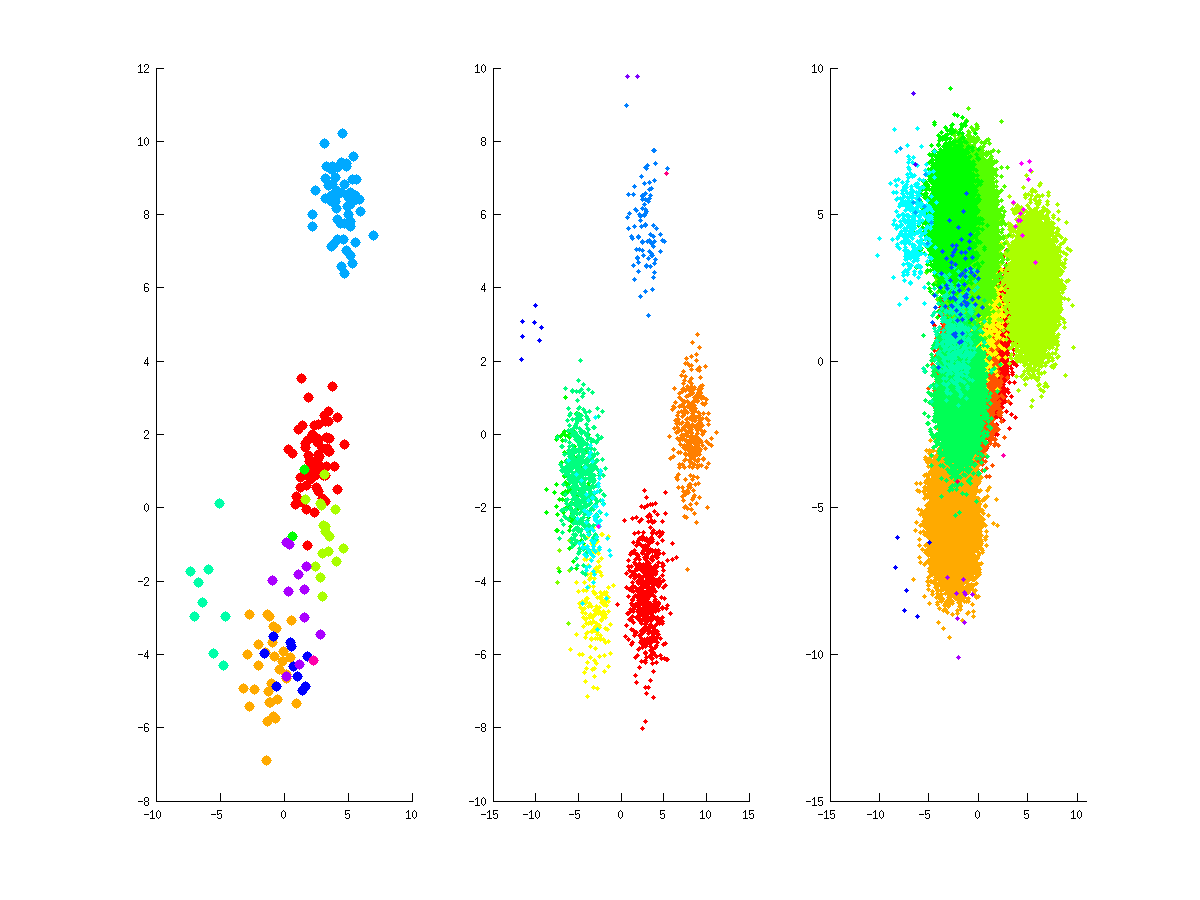
\includegraphics[trim=23mm 0mm 0mm 0mm, clip=true, height=80mm, width=150mm]{2_1_1}
\vspace{-10mm}
\caption{Points and clusterings from the Dirichlet process for $\alpha = 1$,
and $n \in \{200, 2000, 2 \times 10^5\}$.}
\label{fig:2_1_1}
\end{figure}
\begin{figure}[h!]
\centering
\quad\;
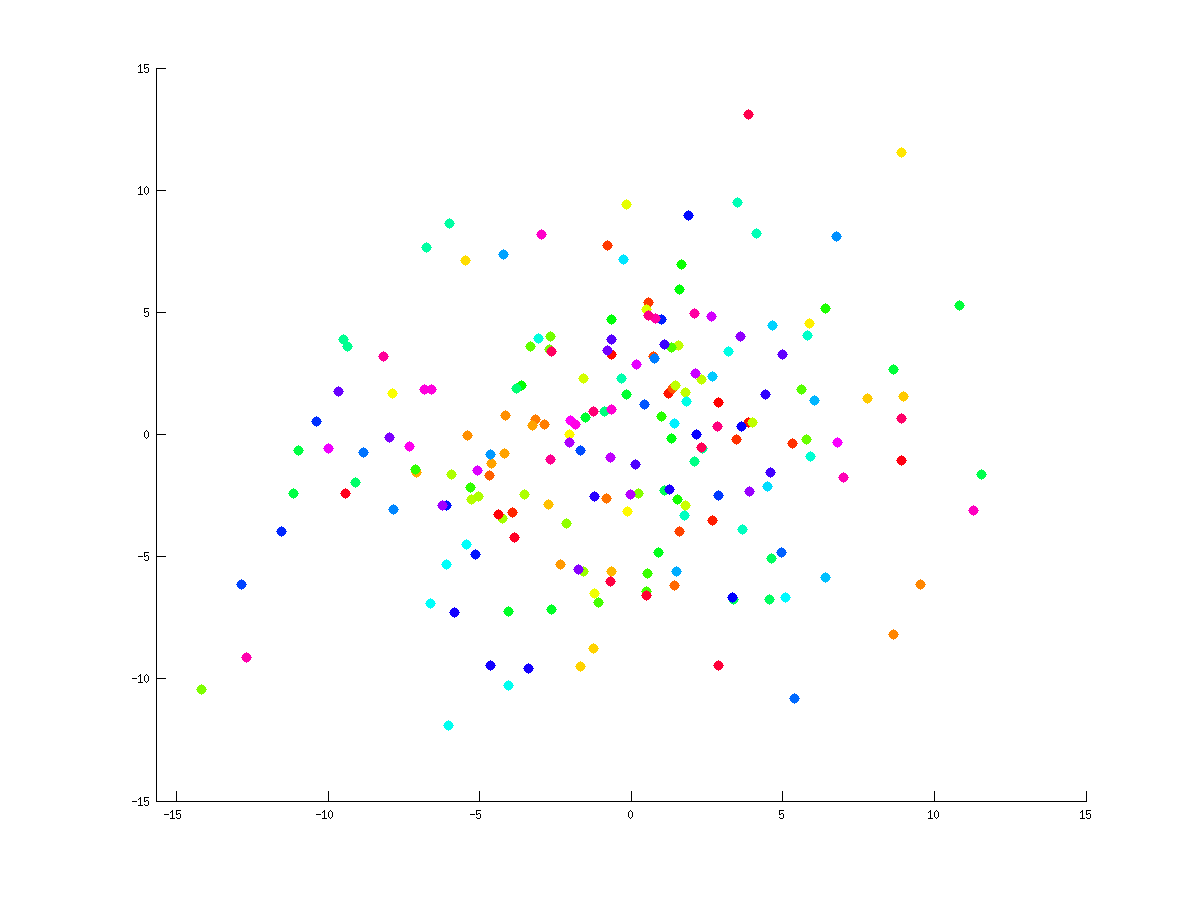
\includegraphics[trim=23mm 0mm 0mm 0mm, clip=true, width=0.6\linewidth]{2_1_2}
\vspace{-8mm}
\caption{Points and clusterings from the Dirichlet process for $\alpha = 400$
and $n = 200$.}
\label{fig:2_1_2}
\end{figure}
\end{enumerate}
\subsection{Inference with Gibbs sampling}
\subsubsection{Conditional distributions (10 points)}
By Bayes' Rule, since, for $i \neq j$, $x_i$ is conditionally independent of
$\mu_{-k}, x_{-i},z_{-i}$ given $\mu_k,z_i = k$, and, without knowing $x_i$,
the distribution of $z_i$ depends only on the distribution of values in
$z_{-i}$,
\begin{align*}
p(z_i = k | \mu, x, z_{-i})
    = C p(x_i | \mu_k, z_i = k) p(z_i = k | \mu, x_{-i}, z_{-i})
 &  = C p(x_i | \mu, x_{-i}, z) p(z_i = k | z_{-i}) \\
 &  = C \frac{n_{-i,k}}{n - 1 + \alpha} p(x_i | \mu, x_{-i}, z),
\end{align*}
where the last line follows from construction of the DPM. Similarly,
\begin{align*}
p(z_i = K_{new} | \mu, x, z_{-i})
 &  = C p(x_i | \mu_k, z_i = K_{new}) p(z_i = K_{new} | \mu, x_{-i}, z_{-i}) \\
 &  = C p(z_i = K_{new} | z_{-i})
        \int p(x_i | \mu_k, z_i = K_{new}, \mu) \pi(\mu) \, d\mu \\
 &  = C \frac{\alpha}{n - 1 + \alpha}
        \int p(x_i | \mu_k, z_i = K_{new}, \mu) \pi(\mu) \, d\mu,
\end{align*}
where we used the Law of Total Probability followed by the construction of the
DPM.

\subsubsection{Implementation (20 points)}
In the case $d = 2$, $F_0 = \mathcal{N}(0, 25I)$, Equation (3) simiplifes to
\begin{align*}
p(\mu_k = u | x,z,\mu_{-k})
    \propto \frac{1}{50\pi} \exp\left( -\frac{\|u\|^2}{50} \right)
        \prod_{i : z_{i = k}} \frac{1}{2\pi}
                        \exp \left(- \frac{\|x_i - \mu\|^2}{2} \right)    \\
    = \frac{1}{25(2\pi)^{n_k + 1}} \exp\left(
        -\frac{\|u\|^2}{50} - \sum_{i : z_{i = k}} \frac{\|x_i - \mu\|^2}{2}
        \right),
\end{align*}
Equation (4) simplifies to
\begin{align*}
p(z_i = k | \mu, x, z_{-i})
    = C\frac{n_{-i,k}}{2\pi n}
        \exp\left( -\frac{\|x_i - \mu_k\|^2}{2} \right),
\end{align*}
and Equation (5) simiplifies to
\begin{align*}
p(z_i = K_{new} | \mu, x, z_{-i})
 &  = C \frac1n
        \int \frac{1}{2\pi} \exp\left( - \frac{\|x_i - \mu_k\|^2}{2} \right)
        \frac{1}{50\pi}\exp\left( -\frac{\|\mu\|^2}{50} \right) \, d\mu.
\end{align*}
This integral is fairly standard and can be computed by completing the square
in the exponent, but I didn't have time to finish this. Consequently the code
below consistently clusters all points into the same cluster, and so I didn't
include a plot of the clustering.

In order to sample new cluster means, we also need the posterior distribution
of $\mu_k$ given $x_i, z_i = k$. Since the conjugate prior of a Gaussian is
Gaussian, a standard formula shows
$\mu_k | x_i, z_i = k \sim \mathcal{N}(\mu, \Sigma)$, where
\[\mu
    = ((25I)\inv + I\inv)\inv(I\inv x_i)
    = \frac{25}{26} x_i
\quad \mbox{ and } \quad
\Sigma
    = ((25I)\inv + I\inv)\inv
    = \frac{25}{26} I.
\]

\subsubsection{Prediction (5 points)}
I didn't have time to finish this part.

\subsubsection*{Code for Section 2.1}
\begin{verbatim}
alpha = 1; n_samples = 2*10^2; d = 2; % data dimension
mu_0 = zeros(1, d); Sigma_0 = 25*eye(d); % mean and covariance of F_0
Sigma = eye(d); % within-cluster variance
assignments = zeros(n_samples, 1); % cluster assignments
for sample=1:n_samples
  % w is a vector of probabilities of each cluster (or a new cluster)
  w = [histc(assignments, 1:max(assignments)); alpha]/(sample - 1 + alpha);
  clust = sum(rand > cumsum(w)) + 1; % sample a cluster according to w
  assignments(sample) = clust; % assign sample to cluster
end
clust_mus = mvnrnd(mu_0, Sigma_0, max(assignments)); % draw cluster means
samples = mvnrnd(clust_mus(assignments, :), Sigma); % draw samples
\end{verbatim}

\newpage
\subsubsection*{Code for Section 2.2}
\begin{verbatim}
B = 1000; % number of burnin samples
T = 100; % number of samples to use
alpha = 1;
load q2;
[n d] = size(x);

% parameters of prior
mu_0 = zeros(1, d);
Sigma_0 = 25*eye(d);
Sigma = eye(d);

Zs = zeros(n, 1);
Mus = zeros(0, d);
for iter = 1:(B + T)
  for sample = 1:n % resample cluster labels for each sample
    for cluster = 1:size(Mus, 1) % compute prob. of x coming from each cluster
      p_clust = (sum(Zs ==  cluster) - (Zs(sample) ==  cluster))/(n - 1 + alpha);
      w(cluster) = p_clust*mvnpdf(x(sample, :), Mus(cluster, :));
    end

    % compute prob of x coming from new cluster
    p_clust = alpha/(n - 1 + alpha);
    w(size(Mus, 1) + 1) = p_clust; % I DIDN'T HAVE TIME TO DERIVE THIS LINE
    % sample cluster label by weight w
    Zs(sample) = sum(rand >= cumsum(w./sum(w))) + 1

    if(Zs(sample) > size(Mus, 1)) % sample a new cluster
      Mus = [Mus; sample_post(x(sample, :), Sigma, mu_0, Sigma_0)];
    end
  end
  for cluster = 1:size(Mus, 1) % resample cluster means for each cluster
    Mus(cluster, :) = sample_post(x(Zs ==  cluster, :), Sigma, mu_0, Sigma_0);
  end
end

% sample from posterior of Gaussian mean given a prior and samples Xs
function mu = sample_post(Xs, Sigma, mu_0, Sigma_0)
  Xs_m = mean(Xs, 1);
  n = size(Xs, 1);
  S = inv(inv(Sigma_0) + n*inv(Sigma));
  m = S*(inv(Sigma_0)*mu_0' + n*inv(Sigma)*Xs_m');
  mu = mvnrnd(m', S);
end
\end{verbatim}
\end{document}
